\scanpage{53}
avec
\[
(5)\qquad\rho_\infty=\tau_1\tau_0,\quad\rho_1=\tau_0\tau_\infty,\quad\rho_0=\tau_\infty\tau_1
\]

La relation avec les ``repères'', en tant que simplexes topologiques de la subdivision barycentrique, est la suivante:

\figure{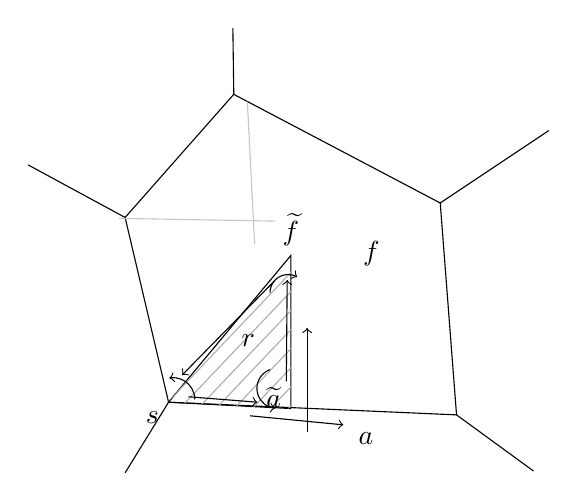
\begin{tikzpicture}[scale=1.15]
\coordinate (s) at (0,0);\coordinate (aa) at (1.35,-.07);\coordinate (ff) at (1.35,1.62);
\draw (s)--(-.48,2.04)--(.72,3.4)--(3,2.2)--(3.18,-.14)--cycle;
\draw (s)--(-.48,-.78) (-.48,2.04)--(-1.55,2.62) (.72,3.4)--(.71,4.13) (3,2.2)--(4.2,3) (3.18,-.14)--(4.03,-.76);
\draw[gray!45,thin] (-.55,2.03)--(1.18,2) (.87,3.32)--(.95,1.75);
\draw (s)--(ff)--(aa)--cycle;
\begin{scope}\clip (s)--(ff)--(aa)--cycle;
\foreach \x in {-1,-.8,...,1.3}{\draw[gray!65,thin] (\x,-.2)--(\x+1.9,1.8);}\end{scope}
\draw[->] (.22,.06)--(.98,0);
\draw[->] (1.3,.23)--(1.31,1.35);
\draw[->] (1.17,1.34)--(.15,.3);
\draw[->] (.29,.03) arc (0:100:.24);
\draw[->] (1.12,.36) arc (110:265:.22);
\draw[->] (1.12,1.21) arc (180:60:.2);
\draw[->] (1.53,-.33)--(1.53,.82);
\draw[->] (.9,-.15)--(1.93,-.25);
\node[below left] at (s) {$s$};\node[left] at (1.35,.05) {$\widetilde a$};
\node[above] at (ff) {$\widetilde f$};\node at (.88,.68) {$r$};\node at (2.24,1.64) {$f$};\node[below] at (2.18,-.23) {$a$};
\end{tikzpicture}}

Le biarc \inserted{associé au repère $r$} a comme orientation tangentielle celle qui \uline{sort} du sommet $s$, comme orientation normale celle qui \uline{entre} dans la face $f$ (``on sort des sommets pour entrer dans la face $f$, en passant par l'arête $a$''). Les trois sommets de $r$ sont le sommet $s=\widetilde s$, le ``centre'' $\widetilde a$ de $a$, et le ``centre'' $\widetilde f$ de $f$, l'orientation de $r$ est celle qui tourne autour de $r$ dans le sens $s\,\widetilde a\,\widetilde f$ (comme le dit la \unsure{notation} image plus bas).

C'est aussi celle pour laquelle l'\deleted{\unsure{flèche}} orientation normale \inserted{de l'arête $a$} indique le sens de rotation direct autour du sommet $s$, \inserted{``origine'' de $a$ pour l'orientation tangentielle choisie)}, et pour laquelle l'orientation tangentielle indique le sens de rotation autour de $f$ (``\unsure{fin extrémité}'' de $a$, pour l'orientation normale du biarc). Les sens de rotation ``directe'' (pour l'orientation définie par $r$) autour des trois sommets de $r$ sont indiqués sur la figure. Sur les patrons formés par les \deleted{triangles} \inserted{simplexes} topologiques $r$, avec les trois sommets écrits comme sur la figure, le sens de l'orientation des \unsure{portions} le long des arêtes $\widetilde s\widetilde a,\,\widetilde a\widetilde f,\,\widetilde f\widetilde s$ \unsure{paraît à rebours} sur les portions des parcours qui tournent autour des sommets

\mspage{52}
